\documentclass{beamer}
\usetheme{Madrid}
\usecolortheme{default}

\title[Social Connections Analysis]
{Effects of Socialization on Mental Health}

\subtitle{STA130 Course Project}

\author[STA130] % (optional, for multiple authors)
{Edie Chen \and Jason Li \and Zain Mahmoud \and Rana Nagash\\
TA Oliver Gatalo\\
Professor Scott Schwartz}

\institute[UofT] % (optional)
{
  STA130: An Introduction to Statistical Reasoning and Data Science\\
  Department of Statistical Sciences\\
  University of Toronto
}

\date[November 2024] % (optional)


\logo{
\includegraphics[height=0.8cm]{logo_uoft}}

\definecolor{uoftblue}{RGB}{6,41,88}
\setbeamercolor{titlelike}{bg=uoftblue}
\setbeamerfont{title}{series=\bfseries}

\begin{document}

\frame{\titlepage}


\section{Introduction}

\begin{frame}
\frametitle{Introduction}
Social interactions play a pivotal role in shaping individual mental health outcomes. It is becoming increasingly easier, especially for teenagers, to connect with their friends virtually from the comfort of their homes. One may argue that this is harmful for their mental health; is this always the case?\\
Through this research, we aim to highlight the difference between physically interacting with community members as opposed to virtually connecting with them. \alert{Canadian Social Connections Survey (CSCS)} to investigate the relationship between various forms of social interactions (physical and non-physical) and how they affect the individuals' mental health states. 
This presentation outlines the variables we're using, our hypotheses, analyses, key findings, and the conclusions we've drawn from these findings.
In this study, we analyze data from the 
\end{frame}


\section{Research questions}

\begin{frame}
\frametitle{Our research questions}

\begin{block}{Question 1}
Do the frequency days where an individual spends at least 5 minutes physically socializing lessen an individual’s degree of depression?
\end{block}

\begin{block}{Question 2}
Does playing online games affect how often you feel depressed, and does going outside with friends counteract that? 
\end{block}

\begin{block}{Question 3}
    Does video chatting with others make one feel less lonely than text messaging? 
\end{block}
\end{frame}
\section{Question 1}
\begin{frame}
\frametitle{Question 1: Variables}

Independent variables:

\vspace{1em}

{\small{\tt CONNECTION\_social\_days\_family\_p7d\_grouped}:\\
days where individuals spent at least 5 minutes socializing with family.}

\vspace{0.5em}

{\small{\tt CONNECTION\_social\_days\_friends\_p7d\_grouped}:\\
days where individuals spent at least 5 minutes socializing with friends.}

\vspace{0.5em}

{\small{\tt CONNECTION\_social\_days\_coworkers\_and\_classmates\_p7d\_grouped}:\\
days where individuals spent at least 5 minutes socializing with co-workers or classmates.}

\vspace{0.5em}

{\small{\tt CONNECTION\_social\_days\_neighbours\_p7d\_grouped}:\\
days where individuals spent at least 5 minutes socializing with neighbours.}

\vspace{1.5em}

Dependent variable:

{\small{\tt WELLNESS\_phq\_score}:\\
metric used to characterize an individual's level of depression on a scale\\
of 0-6.}


\end{frame}


\begin{frame}{Preliminary analysis}
    After keeping only the columns we're interested in and cleaning the data, we were left with 575 rows and 6 columns.
\begin{figure}
    \centering
    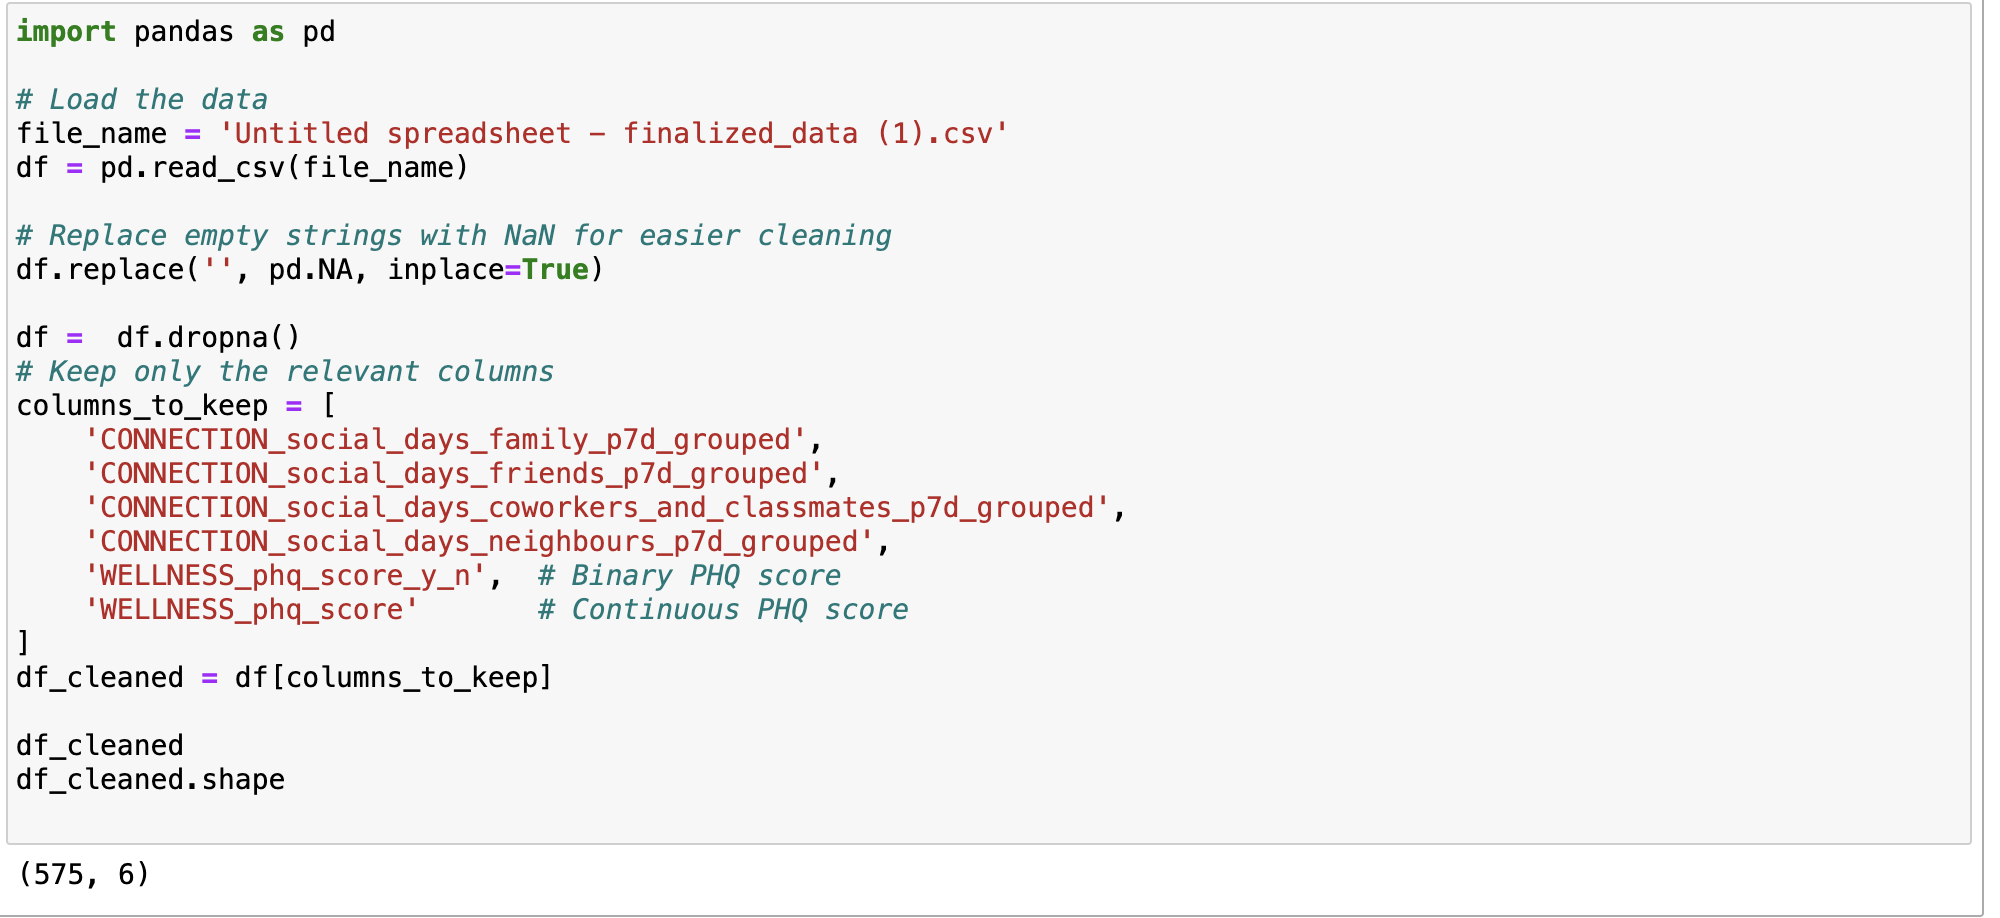
\includegraphics[width=1\linewidth]{image.png}
    \caption{6x575 cleaned dataframe}
    \label{fig:enter-label}
\end{figure}
\end{frame}

\begin{frame}{Preliminary analysis}
    The independent variables were categorical with 4 categories each: 
\begin{figure}
    \centering
    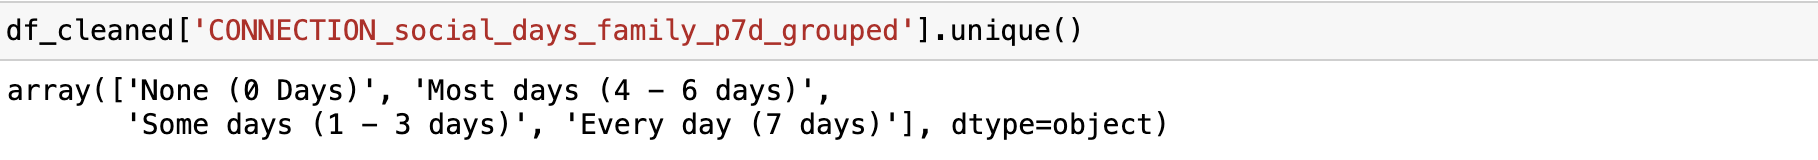
\includegraphics[width=1\linewidth]{image2.png}
    \caption{Unique data entries in one of the columns }
    \end{figure}
    To better analyze the data, we gave each category a numeric value based on the midpoint of the interval. For example, the 'Most days (4-6)' category was assigned 5 (representing the midpoint of the number of days). Then, we added another column to represent the total number of days where each individual spent at least 5 minutes socializing with any one of the groups above using the numeric values we assigned to each category. 
\end{frame}


\begin{frame}{Analysis}
    First, we examined the relationship between the total column and the numeric PHQ score column. We did this by fitting a simple linear regression through the data.
    \begin{columns}
        \column{0.5\textwidth}
        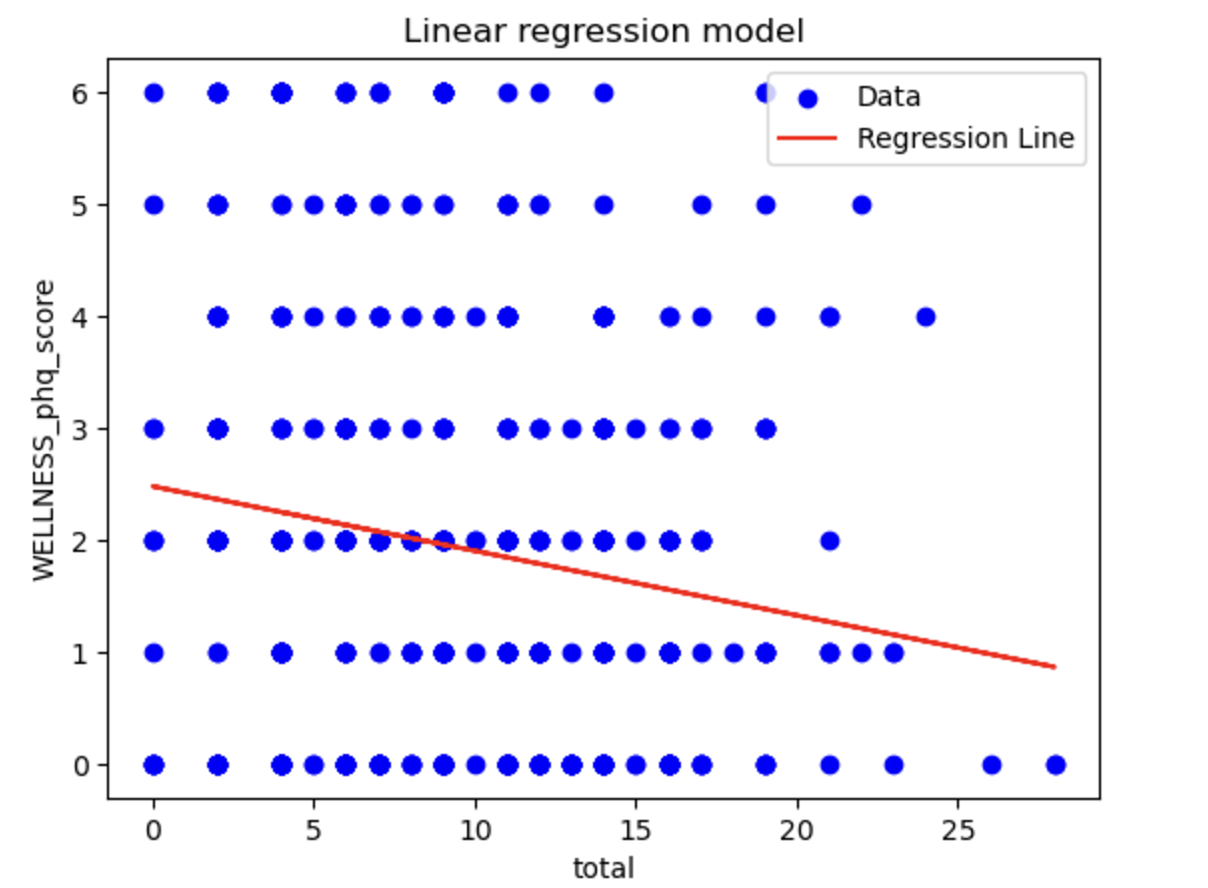
\includegraphics[width=1\linewidth]{model1.png}\\
        \column{0.5\textwidth}
        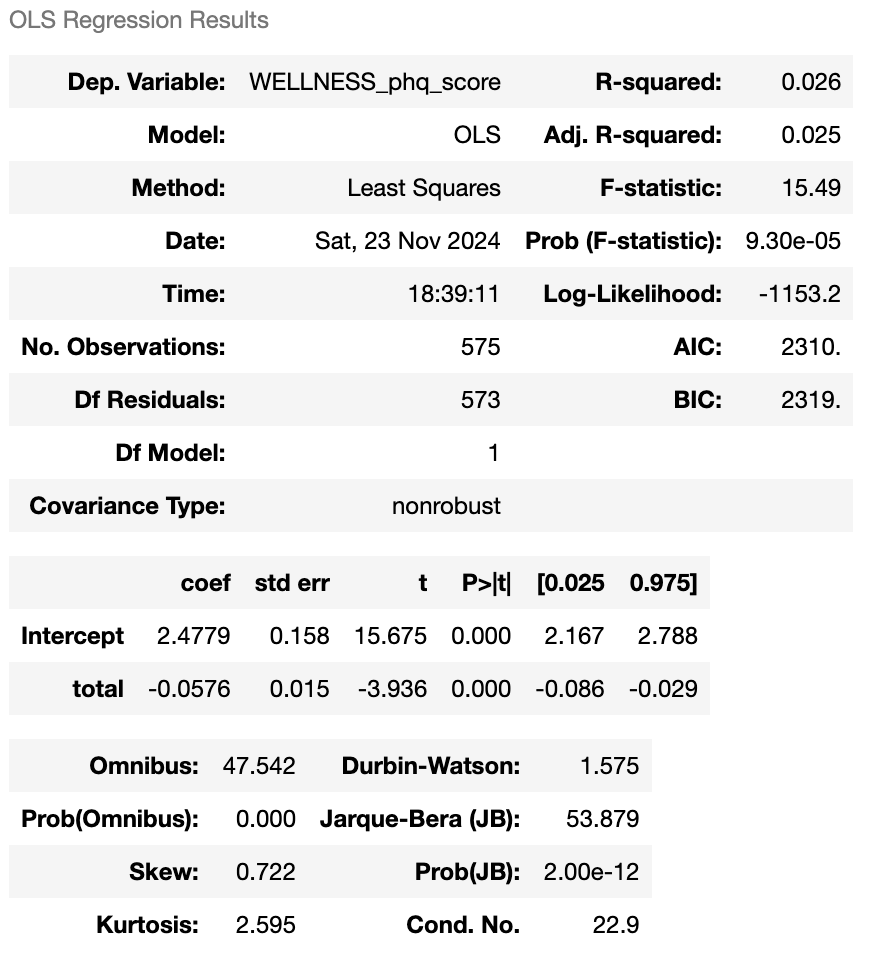
\includegraphics[width=1\linewidth]{summarystats.png}

        
    \end{columns}
\end{frame}

\begin{frame}{Analysis}
    We then created a bootstrapped distribution of model slope coefficients by repeatedly resampling from our original sample and refitting OLS models through the samples. Then, we created a 95\% confidence interval of our bootstrapped coefficients for inference.
    \begin{figure}
        \centering
        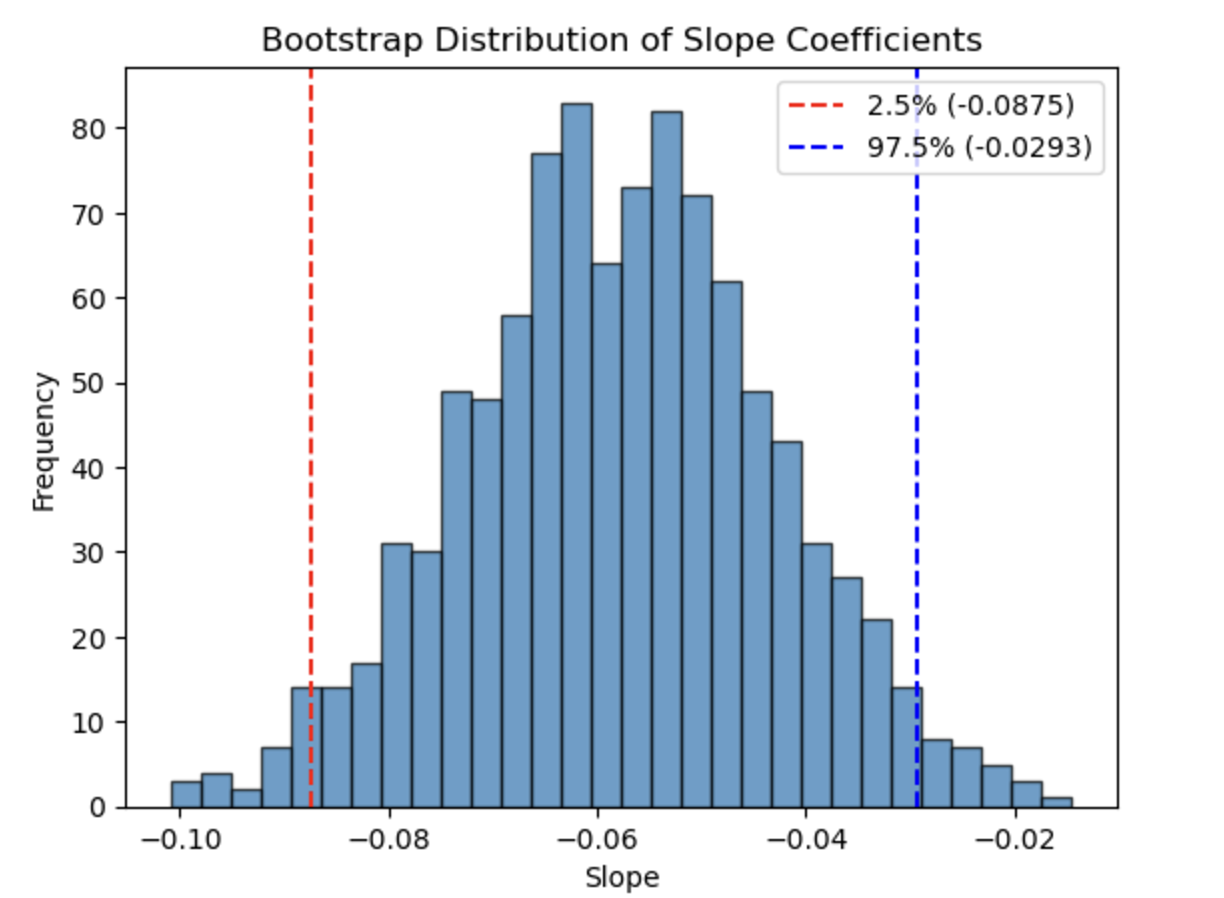
\includegraphics[width=0.5\linewidth]{95CI.png}
        \caption{95\% confidence interval}
        \label{fig:enter-label}
    \end{figure}
\end{frame}

\begin{frame}{Summary and conclusion}
The confidence interval we constructed only contained negative slopes between $-0.0875$ and $-0.0293$ and so we can conclude with 95\% confidence that the true value of the slope coefficient lies in that interval. This means that as the number of days where an individual spends at least 5 minutes socializing increases, the average depression score decreases. However, the values of the slopes are very small and so the effect of socializing on depression scores is minuscule (albeit negative).
    
\end{frame}






% Jason

\section{Question 2}

\begin{frame}
    \frametitle{Question 2: Variables}
    
    Independent variables:
    
    \vspace{1em}
    
    {\small{\tt CONNECTION\_activities\_onlinegames\_p3m}:\\
    how often an individual has played online games in the past 3 months}
    
    \vspace{0.5em}
    
    {\small{\tt CONNECTION\_activities\_walk\_p3m}:\\
    how often an individual has gone on a walk with friends in the past 3 months}
    
    \vspace{1.5em}
    
    Dependent variable:

    \vspace{1em}
    
    {\small{\tt WELLNESS\_malach\_pines\_burnout\_measure\_depressed}:\\
    how often an individual feels depressed}
    
    
\end{frame}


\begin{frame}
    \frametitle{Cleaning data}

    First, I want to assign numbers to the ordinal categories of how often an individual feels depressed.

    I will just use the consecutive numbers 0 (never) through 5 (always).

    \begin{figure}
        \centering
        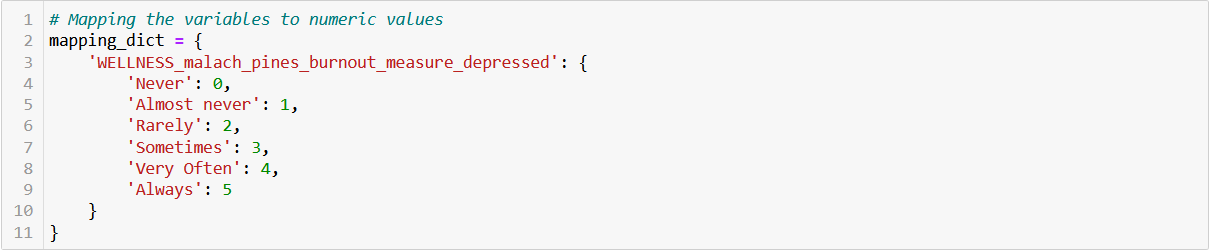
\includegraphics[width=0.8\linewidth]{jason_depressionvalues.png}
    \end{figure}

    After renaming variables, removing empty values, etc., this is what my DataFrame looks like.

    {\tiny The boolean values True are whenever the categorical values are not never/not in the past three months.}

    \begin{figure}
        \centering
        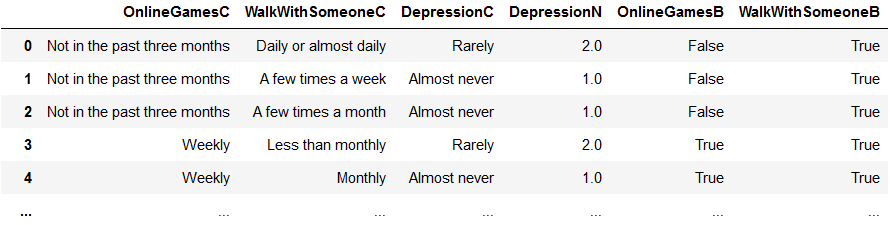
\includegraphics[width=0.7\linewidth]{jason_dfpreview.png}
    \end{figure}
    
\end{frame}

\begin{frame}
    \frametitle{Bar plot}

    \begin{figure}
        \centering
        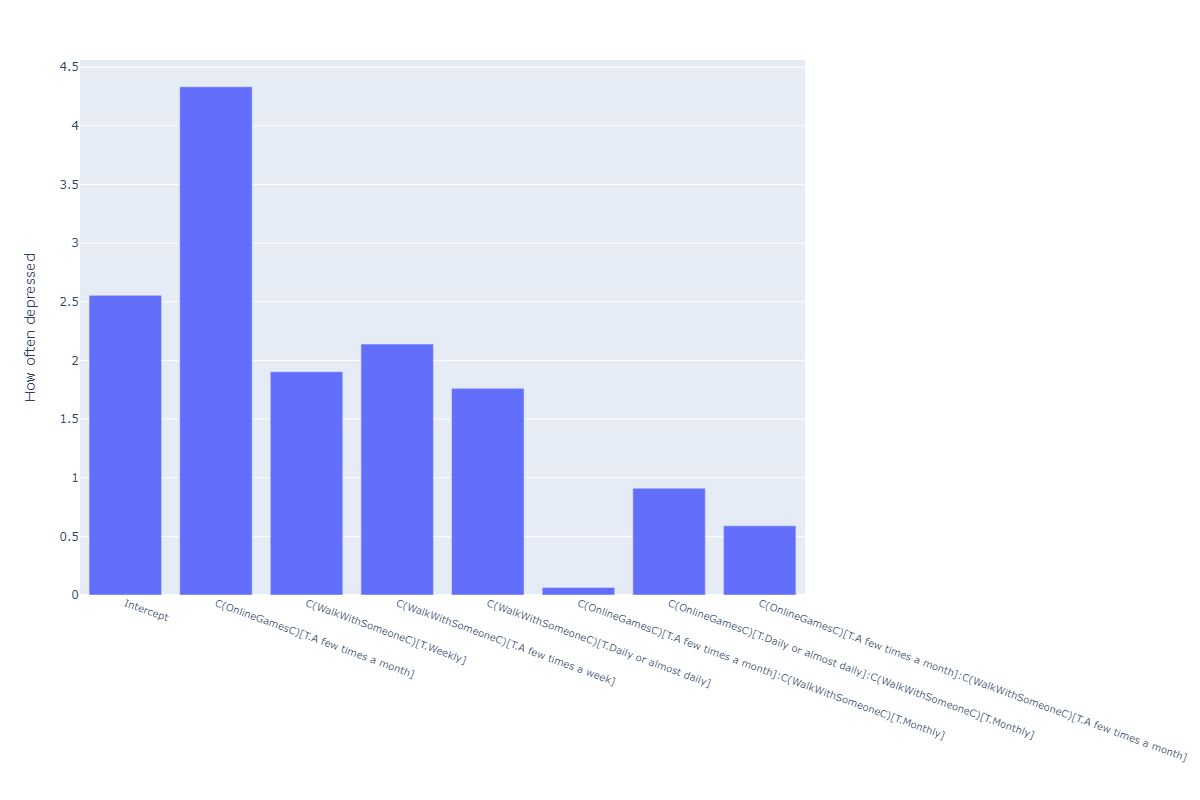
\includegraphics[width=1\linewidth]{jason_barplot.png}
    \end{figure}

\end{frame}


\begin{frame}

\frametitle{Regression}

I will perform a linear regression, with interactions. I will retain only the outcomes with a p-value $\geq 0.05$ for simplicity.

\begin{figure}
    \centering
    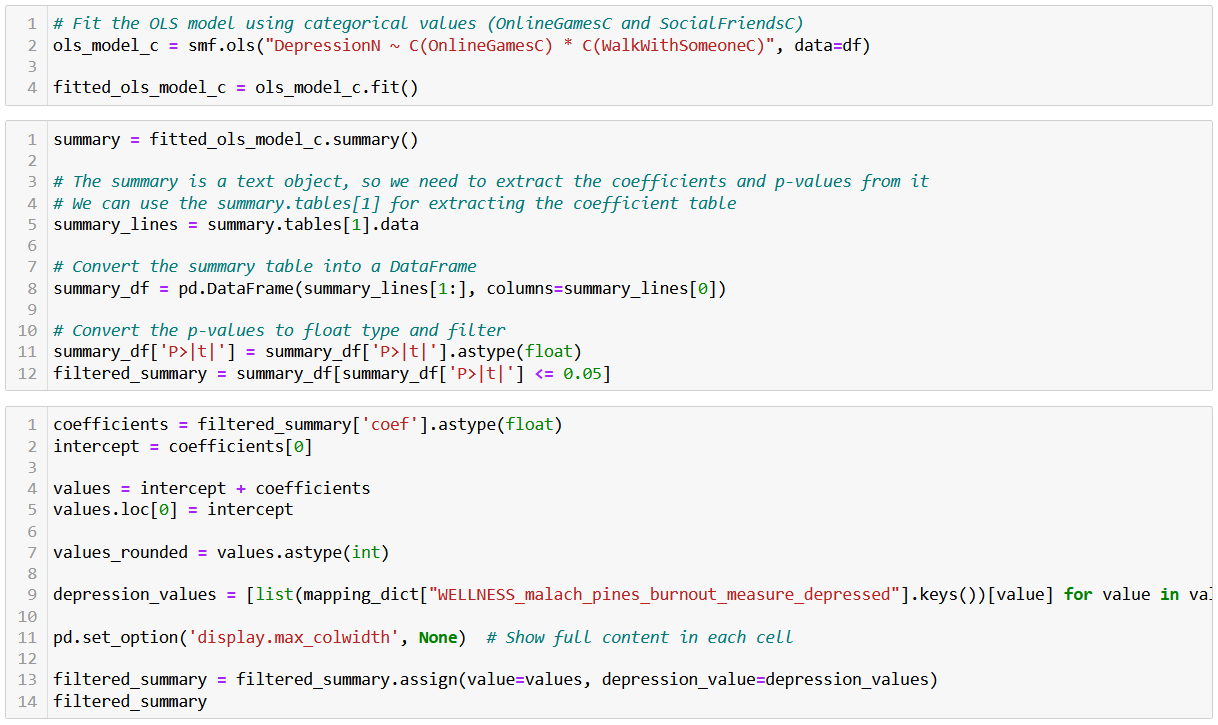
\includegraphics[width=0.6\linewidth]{jason_regression.png}
    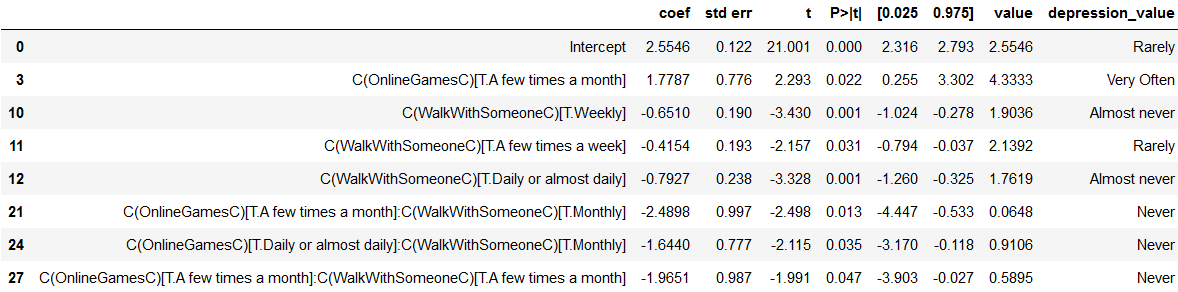
\includegraphics[width=0.6\linewidth]{jason_regressionoutcome.png}
\end{figure}

\end{frame}







\section{Question 3}
%ADD YOUR FRAMES BELOW
\begin{frame}{Question 2 Variables}

Does video chatting with others make one feel less lonely than text messaging others?\\

\textbf{Independant Variables:}\\

Video chatted with friends/family in the past 3 months:\\

Texted or messaged someone in the past 3 months:\\

Options:
\begin{itemize}
    "Not in the past three months",
    "Less than monthly",
    "Monthly",
    "A few times a month",
    "Weekly",
    "A few times a week",
    "Daily or almost daily"
\end{itemize}

\textbf{Dependant Variables:}\\

How many days felt lonely in the past week:\\

Options:
\begin{itemize}
'None of the time (e.g., 0 days)': 0,
    'Rarely (e.g. less than 1 day)': 0.5,
    'Some or a little of the time (e.g. 1-2 days)' : 1.5,
    'Occasionally or a moderate amount of time (e.g. 3-4 days)': 3.5,
    'All of the time (e.g. 5-7 days)': 6
\end{itemize}
\end{frame}

\begin{frame}{Assumptions}
Converting the categorical variable to numerical values makes it not completely accurate since it assumes an exact number of days that they feel lonely\\


How many days people feel lonely in a week is not reflective of how lonely they feel on average\\
\end{frame}

\begin{frame}{Visualization of the Raw Data}


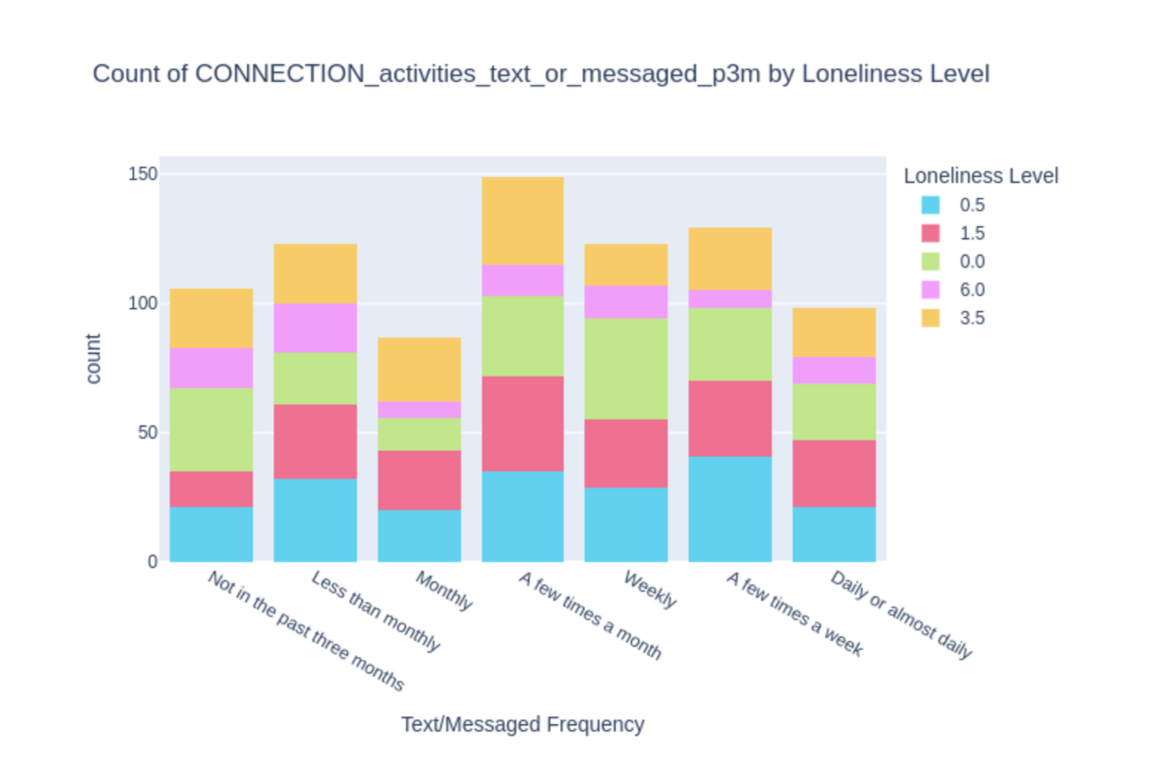
\includegraphics[width=0.5\linewidth]{Screenshot 2024-11-28 at 12.28.29 PM.png}
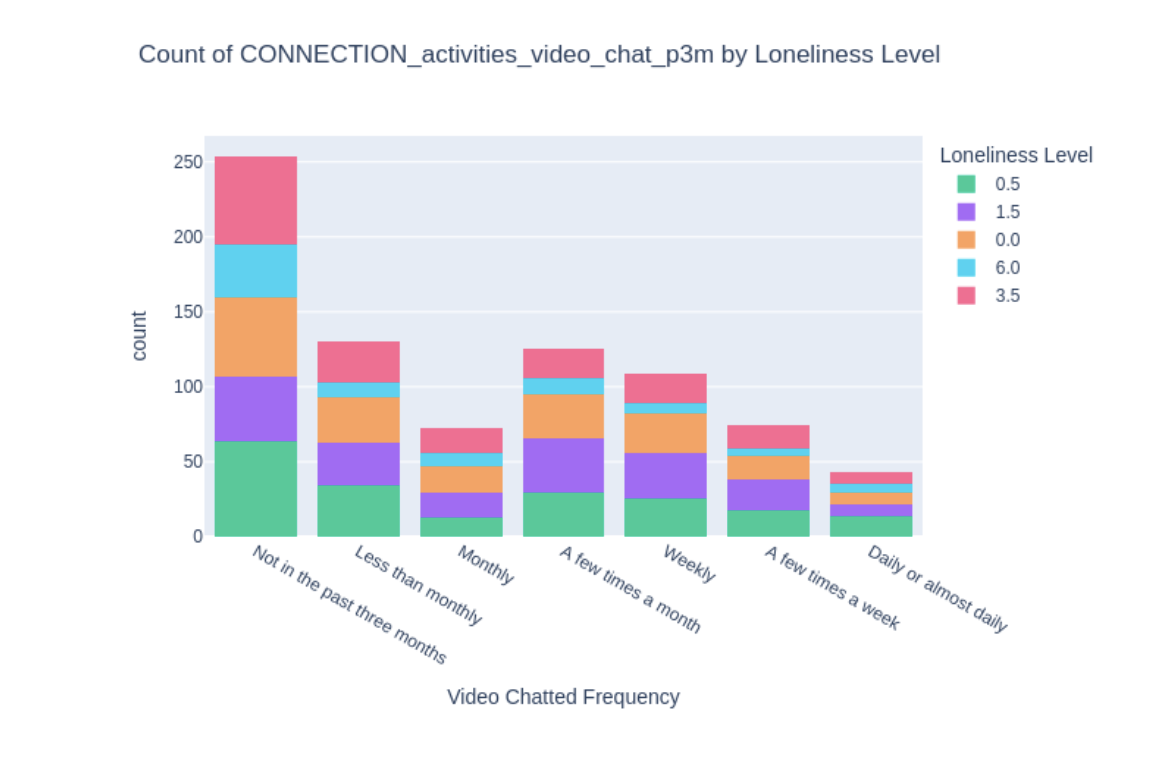
\includegraphics[width=0.5\linewidth]{Screenshot 2024-11-28 at 12.31.04 PM.png}


\end{frame}

\begin{frame}{Simple Linear Regression & Data Wrangling}

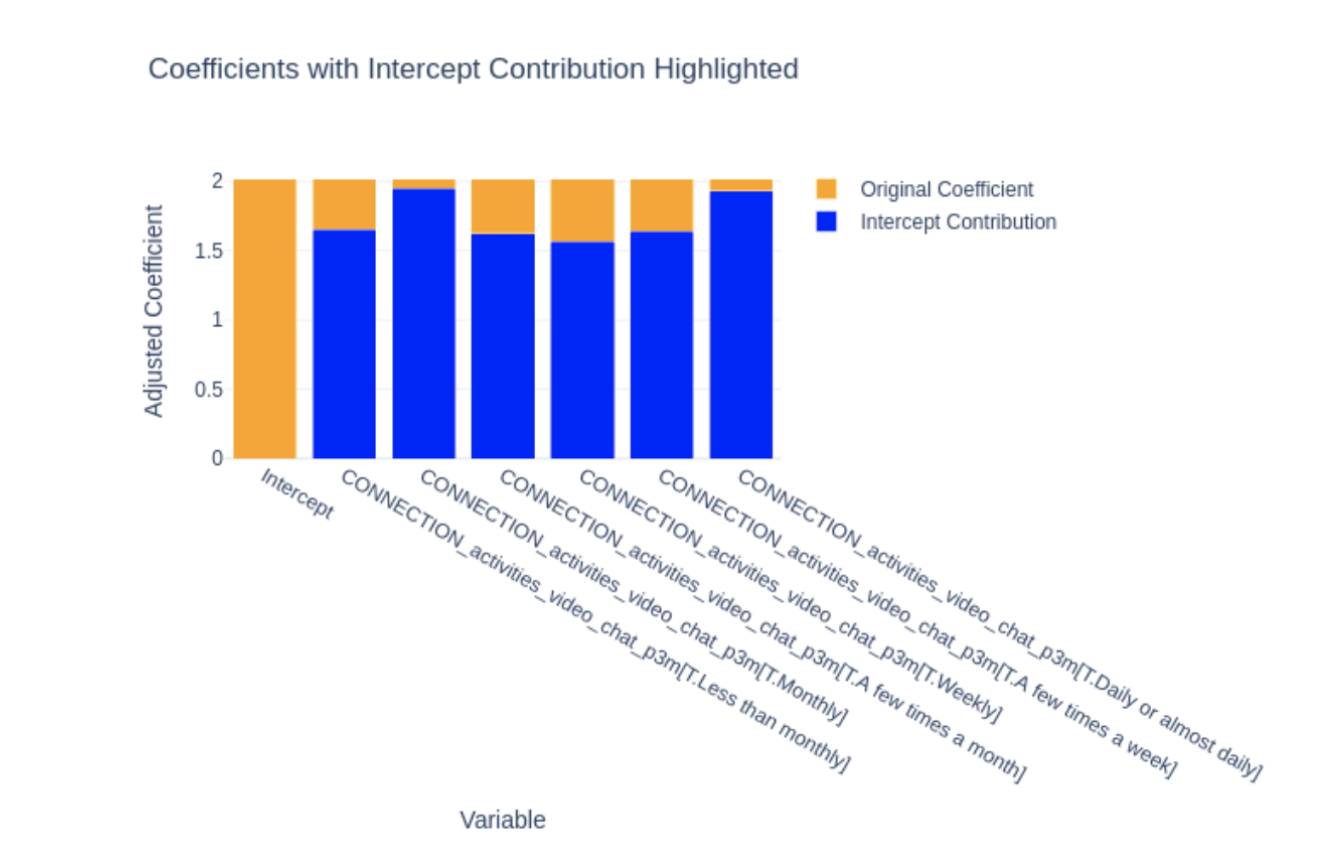
\includegraphics[width=0.5\linewidth]{Screenshot 2024-11-28 at 12.32.21 PM.png}

We first tried to analyse the 2 factors separately with simple linear regression\\
The fitting of the model was poor (R square = 0.01)\\
So we decide to analyse with a  multilinear regression model\\
\end{frame}

\begin{frame}{Final Result & Analysis}


Multilinear Regression with Heat Map Visualization.\\
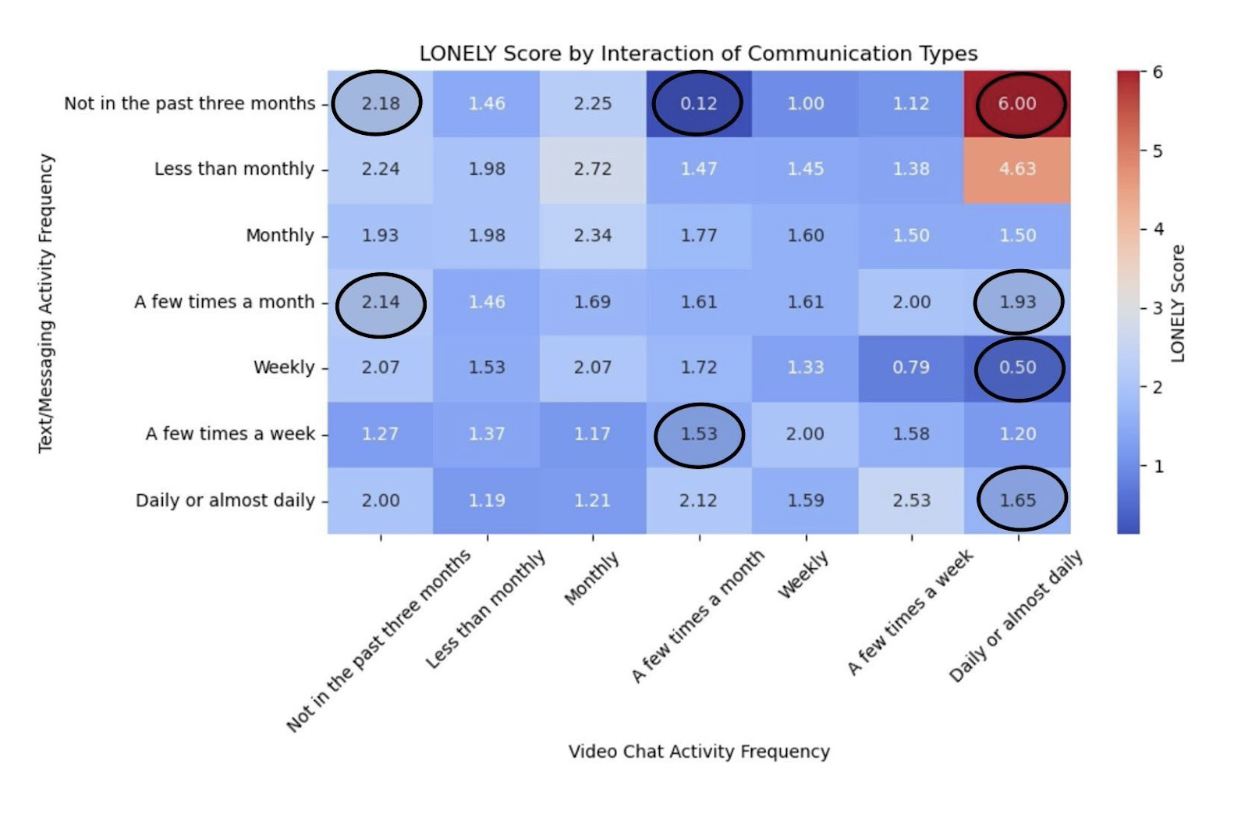
\includegraphics[width=0.5\linewidth]{image4.png}


The circled ones are the final value which got a p value lower than 0.05 (meaningful).\\
The r-squared is 0.065 for the multilinear regression\\
\end{frame}

\begin{frame}
\textbf{Conclusions:}\\
Video chatting daily or almost daily without texting in the past three months leads to high levels of loneliness\\
Video chatting daily or almost daily and texting weekly leads to low levels of loneliness\\
Video chatting a few times a month and texting a few times a month also leads to low levels of loneliness\\

*Reminder that this is not completely accurate due to assumptions mentioned previously\\
\end{frame}

\section{Question 3}
%ADD YOUR FRAMES BELOW
\begin{frame}{Frame Title}
    
\end{frame}

\begin{frame}{Conclusion}

\textbf{Connections}\\
Aim to analyze how socializing in different forms affects people’s mental health\\
branched off into 2 directions to find out the effect of  interaction when it's offline or online.\\

\textbf{Findings}\\ 
Socializing and Depression:\\
The average depression score decreases when physical socialization $>=$ 5 min/day\\
Depression levels also drop when taking a walk with others.\\
Playing video games, however, may have an opposing effect on level depression.\\
Socializing and Loneliness:\\
Contacting others a few times a month via video chat and test seems to reduce loneliness the most.\\

    
\end{frame}

\begin{frame}{Future Directions & Acknowledgments}
\textbf{Acknowledgments:}\\
We would like to thank Dr. Kiffer Card and Ms. Christine Ovcaric for providing this valuable opportunity. Special thanks to Prof. Schott, our TA, and all the teaching assistants for their guidance and support throughout the project.
\end{frame}

\end{document}